\documentclass[10pt,a4paper]{article}
\usepackage[margin=0.78in]{geometry}
\usepackage[T1]{fontenc}
\usepackage[utf8]{inputenc}
\usepackage{lmodern}
\usepackage{microtype}
\usepackage{amsmath,amssymb,booktabs,graphicx}
\usepackage{float}
\usepackage{xcolor}
\usepackage{listings}
\usepackage{hyperref}
\usepackage{enumitem}
\hypersetup{colorlinks=true,linkcolor=blue,citecolor=blue,urlcolor=blue}
\lstset{
  language=Python,basicstyle=\ttfamily\footnotesize,
  keywordstyle=\color{blue!70!black},commentstyle=\color{gray!80!black},
  stringstyle=\color{green!40!black},showstringspaces=false,
  breaklines=true,frame=single,columns=fullflexible,
  xleftmargin=1em,framexleftmargin=0.7em
}
\setlength{\parskip}{0.35em}
\setlength{\parindent}{0pt}
\title{\textbf{A Reproducible Comparison of Random and k-means++ Initialisation}\\
\large Lloyd's Algorithm on Synthetic Data and MNIST}
\author{Statistical Methods for Machine Learning, DSE}
\date{VIOLA AWOR}

\begin{document}
\maketitle
\begin{abstract}
This report implements Lloyd's k-means algorithm from scratch and compares uniform random and k-means++ initialisation. Four benchmark datasets are used: separated and overlapping two-dimensional Gaussian blobs, a 100-dimensional synthetic problem, and a 3,000-image subset of MNIST. Each method is run 60 times with controlled seeds. The evaluation examines within-cluster sum of squares (inertia), convergence iterations, run-to-run stability, external ARI/NMI against reference labels, and non-parametric tests of run-level inertia with Holm correction and bootstrap confidence intervals. On the separated and high-dimensional synthetic problems, k-means++ substantially reduces mean inertia and run-to-run variability; on overlapping blobs and MNIST, the observed mean improvement is small and not statistically significant at the 5\% level. This contrast illustrates that better seeding is most useful when poor initial centres can trap Lloyd's method in markedly inferior local minima, but it does not guarantee a better final partition on every dataset or seed.
\end{abstract}
\tableofcontents
\newpage

\section{Aim and scope}
The aim is to study how initialisation affects the outcome of k-means, not to build a digit classifier. The implementation and experiments compare two choices for the initial $k$ centres: uniform selection of distinct observations and the distance-weighted k-means++ procedure \cite{arthur2007kmeans}. Both use the same Lloyd assignment/update algorithm, stopping tolerance, number of clusters, and input data. The principal question is whether k-means++ yields lower final squared error and more reproducible partitions across random seeds.

K-means is an unsupervised method: it receives feature vectors $X$ and a chosen number of clusters $k$, but not class labels when fitting. Therefore, a conventional train/test classification split and classification accuracy are not appropriate for this experiment. Here $k=5$ is fixed from the synthetic data-generating design and $k=10$ is chosen a priori for MNIST's ten digit categories; this does not test automatic selection of $k$. MNIST labels are only used after each fit to calculate external evaluation scores. No supervised learning or held-out prediction claim is made.

\section{Data acquisition and exploration}
\subsection{Datasets and rationale}
The experiments use four deliberately different settings. The three synthetic datasets provide known, controlled data-generating processes and isolate separation, overlap, and feature dimensionality. MNIST adds a real image benchmark in which Euclidean clusters need not correspond exactly to human-defined digit classes.
\begin{table}[H]
\centering\small
\caption{Benchmark inputs and why each was included. Synthetic ground-truth labels are available from the generator but are not used to fit k-means.}
\begin{tabular}{p{2.25cm}p{2cm}p{2.1cm}p{2.3cm}p{4.0cm}}
\toprule
Dataset & $n$ & Features & $k$ & Purpose and preprocessing\\
\midrule
Separated blobs & 1,500 & 2 & 5 & Low-noise, visually interpretable reference case; Gaussian blobs, standard deviation 0.75.\\
Overlapping blobs & 1,500 & 2 & 5 & Tests ambiguity and local minima; standard deviation raised to 2.4 and centre range narrowed.\\
High-dimensional blobs & 1,500 & 100 & 5 & Tests the same algorithm when many features contribute to Euclidean distance; standard deviation 1.5.\\
MNIST subset & 3,000 & 784 & 10 & Real grayscale handwritten digits; tests a moderate image-clustering workload using pixel intensities.\\
\bottomrule
\end{tabular}
\end{table}

The synthetic cases are generated with \texttt{sklearn.datasets.make\_blobs}, using seed 42 \cite{scikitlearn}. The separated data use two features, five centres, \texttt{cluster\_std=0.75}, and centre range $[-12,12]$. The overlapping variant uses \texttt{cluster\_std=2.4} and centre range $[-8,8]$. The high-dimensional data use 100 features and \texttt{cluster\_std=1.5}. For these synthetic inputs, each feature has the same units by construction, so no additional standardisation is applied.

MNIST is retrieved with \texttt{fetch\_openml("mnist\_784", version=1, as\_frame=False)}. The repository contains OpenML's cached metadata and the compressed ARFF data file under \texttt{data/openml/}; the local file modification time is 26 October 2026 at 15:46:11 +01:00. This filesystem timestamp is the best available local record of cache acquisition, not an independently verified download log. The upstream dataset is MNIST version 1 (OpenML data id 554) \cite{lecun1998mnist,openmlmnist}. The loader selects 3,000 distinct rows using \texttt{RandomState(42)} and scales byte intensities from $[0,255]$ to $[0,1]$ by division by 255. This is range scaling, not z-score standardisation. The chosen subset is reproducible and small enough for repeated trials; it is not stratified, so its digit proportions may differ slightly from the full dataset.
In code, the data-loading and pixel-scaling operations are:
\begin{lstlisting}
mnist = fetch_openml("mnist_784", version=1, as_frame=False,
                     data_home="./data", parser="liac-arff")
X, y = mnist.data.astype(np.float64), mnist.target.astype(int)
rng = np.random.RandomState(42)
indices = rng.choice(len(X), size=3000, replace=False)
X_subset, y_subset = X[indices] / 255.0, y[indices]
\end{lstlisting}

\subsection{Exploratory analysis}
The notebook generates two-dimensional scatter plots for the synthetic blobs and projects the MNIST subset to two dimensions with principal component analysis (PCA) and t-distributed stochastic neighbour embedding (t-SNE) \cite{jolliffe2002pca,maaten2008tsne}. Figure~\ref{fig:mnist-projections} reproduces the notebook's paired MNIST visualisation, colouring observations by their reference digit labels to show how the projections relate to known classes. PCA is a linear projection that exposes directions of greatest global variance; its first two axes explain the variance fractions indicated on the plot. t-SNE is a nonlinear neighbourhood embedding, configured with two components, perplexity 30, and random seed 42. The embedding coordinates and axis scales have no direct metric interpretation.

These are exploratory displays only: class labels are used for colour after embedding and are not inputs to PCA, t-SNE, or k-means fitting. The clustering benchmark still fits k-means on all 784 scaled pixel features; the two-dimensional projections do not change the reported inertia or external scores. PCA and especially t-SNE can distort distances, global geometry, cluster sizes, and gaps between apparent groups, so visual separation is not treated as quantitative evidence of clustering quality.
\begin{figure}[H]
\centering
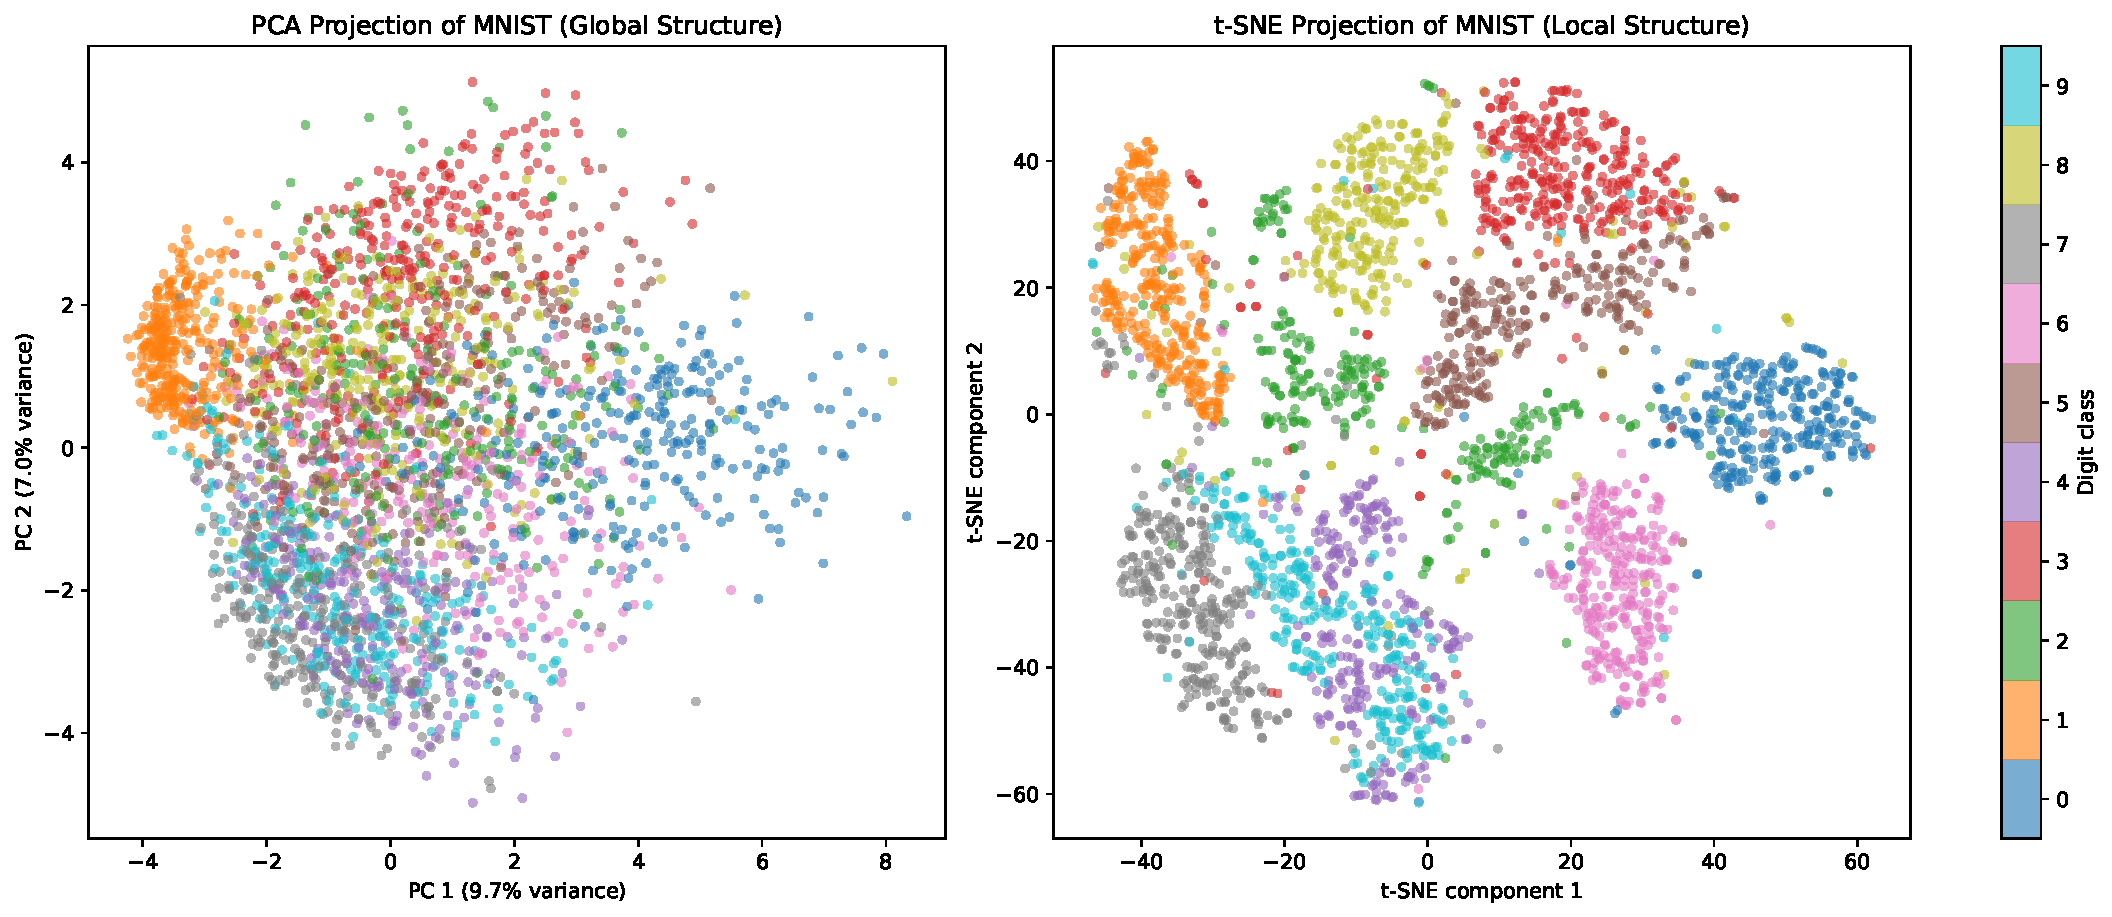
\includegraphics[width=\textwidth]{figures/mnist_pca_tsne.pdf}
\caption{Exploratory projections of the same 3,000-image MNIST subset used in the benchmark. Colours show reference digit class for interpretation only. PCA is linear and t-SNE emphasises local neighbourhood structure; neither projection was used as the clustering feature space.}
\label{fig:mnist-projections}
\end{figure}

\section{Methodology and implementation}
\subsection{Objective and Lloyd iterations}
For observations $x_i\in\mathbb{R}^d$, assignments $z_i\in\{1,\ldots,k\}$, and centres $\mu_j$, k-means minimises the within-cluster sum of squared Euclidean distances:
\[
\Phi(z,\mu)=\sum_{i=1}^{n}\lVert x_i-\mu_{z_i}\rVert_2^2.
\]
Lloyd's algorithm alternates two computations:
\[
z_i\leftarrow\arg\min_{j\in\{1,\ldots,k\}}\lVert x_i-\mu_j\rVert_2^2,
\qquad
\mu_j\leftarrow\frac{1}{|C_j|}\sum_{i:z_i=j}x_i.
\]
The assignment step minimises the objective over labels for fixed centres; the update step minimises it over each centre for fixed labels. Thus each exact step cannot increase inertia. With finitely many possible assignments and deterministic tie handling, the procedure terminates at a fixed point (a local optimum), not necessarily the global optimum. Its result depends on initial centres.

\subsection{Initialisation and theoretical motivation}
Uniform random initialisation selects $k$ distinct observations without replacement. In k-means++, the first centre is sampled uniformly; each subsequent point $x$ is selected with probability proportional to $D(x)^2$, where $D(x)$ is its distance to the nearest already selected centre. This $D^2$-sampling favours points poorly represented by the current seeds and aims to spread the starting centres.

The principal theoretical guarantee is on the \emph{initial} potential: for the standard k-means++ procedure, the expected potential is at most $8(\ln k+2)$ times the optimal $k$-means potential \cite{arthur2007kmeans}. This is an expectation over initialisation, not a guarantee that every run finds the global optimum, nor a bound on the final Lloyd solution. The experiment tests that practical distinction.

\subsection{Distance calculation, stopping and edge cases}
The implementation evaluates squared distances without forming an $n\times k\times d$ difference array, using
\[
\lVert x-\mu\rVert^2=\lVert x\rVert^2-2x^\top\mu+\lVert\mu\rVert^2.
\]
It precomputes $\lVert x_i\rVert^2$ once per fit, computes the matrix product $X\mu^\top$, and clips tiny negative values caused by floating-point rounding to zero. Iteration stops when the Frobenius norm of the change in all centres is below $10^{-4}$ or after 300 iterations. Empty clusters are reseeded to the observation with largest current nearest-centre squared distance; the number of such fixes is tracked by the estimator.

The following excerpt shows the core numerical computation and the objective calculation (from \texttt{src/kmeans.py}):
\begin{lstlisting}
c_sq = np.sum(centers**2, axis=1, keepdims=True).T
dist_sq = np.dot(X, centers.T)
dist_sq *= -2.0
dist_sq += x_sq
dist_sq += c_sq
np.maximum(dist_sq, 0.0, out=dist_sq)
labels = np.argmin(dist_sq, axis=1)
# After the final centre update:
inertia = float(np.sum(np.min(final_dist_sq, axis=1)))
\end{lstlisting}

The seeding calculation samples proportionally to cumulative squared distances; a compact version of the computation is:
\begin{lstlisting}
total_mass = float(np.sum(min_sq))
cum_mass = np.cumsum(min_sq)
cutoff = rng.uniform(0.0, total_mass)
next_idx = int(np.searchsorted(cum_mass, cutoff))
centers[j] = X[next_idx]
new_sq = x_sq.ravel() - 2.0 * np.dot(X, centers[j]) + np.sum(centers[j]**2)
np.minimum(min_sq, new_sq, out=min_sq)
\end{lstlisting}
The repository clips the updated distance array to zero before taking the elementwise minimum and bounds the sampled index to a valid row. If every point has zero distance to a selected centre, the implementation falls back to a uniformly sampled point.

The Lloyd update and stopping computation are shown below. The mean is the least-squares-optimal centre for a fixed cluster; empty clusters use the farthest currently represented point as a reseed:
\begin{lstlisting}
dist_sq = self._compute_sq_distances(X, self.centroids, x_sq)
labels = np.argmin(dist_sq, axis=1)
for c_idx in range(self.k):
    mask = labels == c_idx
    if np.any(mask):
        new_centroids[c_idx] = np.mean(X[mask], axis=0)
    else:
        farthest_idx = np.argmax(np.min(dist_sq, axis=1))
        new_centroids[c_idx] = X[farthest_idx]
shift = float(np.linalg.norm(new_centroids - prev_centroids))
if shift < self.tol:
    break
\end{lstlisting}

\section{Experiment design and evaluation}
\subsection{Repeated-run protocol}
The definitive results in \texttt{experiments/results.json} are produced by \texttt{experiments/run\_experiments.py}. For each of the four fixed datasets, each initialisation is evaluated on 60 seeds, 2000 through 2059, in parallel. Each trial uses the same $k$ for both initialisation schemes. Dataset generation and MNIST subsampling use seed 42; the trial seeds control initial-centre sampling. This is repeated random-start evaluation on fixed data, not cross-validation or a train/test experiment. Fitting uses only feature matrix $X$; reference labels are passed to the scoring function only after fitting.

The recorded measurements are final inertia, Lloyd iteration count, wall-clock runtime, and pairwise adjusted Rand index (ARI) between the partitions from all run pairs. ARI measures agreement between two partitions while correcting for chance; its value of 1 indicates identical partitions, while values near 0 indicate chance-level agreement. Here it measures \emph{stability across runs}. In addition, after fitting only on $X$, each run's predictions are scored against synthetic generator labels or MNIST digit labels using external ARI and normalized mutual information (NMI). These reference labels are never supplied to the estimator, used to choose centres, or used to select hyperparameters. External scores assess correspondence to known categories, not the k-means objective.

The script runs a one-sided Mann--Whitney U test ($H_1$: k-means++ inertias are stochastically lower than random-init inertias) for each dataset and a Levene test ($H_0$: equal variances). The four primary Mann--Whitney p-values are corrected together using Holm's step-down procedure to control family-wise error at $\alpha=0.05$. Levene tests are secondary and reported unadjusted. A 95\% percentile bootstrap interval for the difference in mean inertia (k-means++ minus random) is calculated from 20,000 independent resamples of the two sets of 60 initialisation runs. This interval and the hypothesis tests quantify uncertainty over initialisation on each fixed dataset; they do not capture dataset-to-dataset uncertainty. Because repeated runs can converge to identical solutions, inferential results should be interpreted as conditional on the fixed data and protocol.

\subsection{Expected behaviour}
The expected qualitative outcome is that k-means++ often avoids very poor starting configurations and therefore has lower inertia and fewer iterations, especially when well-separated components make a good initial spread meaningful. The expected advantage can diminish when blobs overlap strongly or when the pixel-space geometry of MNIST does not align well with digit categories. Both methods optimise the same non-convex objective and can reach different local minima. There is no prespecified expected numeric inertia; the correct comparison is within each dataset, because inertia scales with sample count, feature count, and feature magnitude.

\section{Results}
\subsection{Summary of measured outcomes}
Table~\ref{tab:results} gives mean inertia and standard deviation across 60 trials, mean iterations, pairwise ARI stability, and external label scores. Table~\ref{tab:spread} gives the inertia ranges, interquartile ranges, bootstrap intervals, and adjusted primary test results. Inertia should be compared only within a dataset. Lower inertia and higher ARI/NMI are preferable for their respective measures.
\begin{table}[H]
\centering\scriptsize
\caption{Results over 60 starts per initialisation. Inertia and external scores are mean $\pm$ standard deviation; stability is mean pairwise ARI across runs.}
\label{tab:results}
\resizebox{\textwidth}{!}{%
\begin{tabular}{llrrrrr}
\toprule
Dataset & Initialisation & Inertia & Iterations & ARI stability & External ARI & External NMI\\
\midrule
Separated & Random & $5208.6\pm4028.8$ & 8.92 & 0.753 & $0.822\pm0.145$ & $0.910\pm0.072$\\
 & k-means++ & $2665.1\pm1874.0$ & 5.50 & 0.857 & $0.903\pm0.130$ & $0.950\pm0.061$\\
Overlapping & Random & $12914.1\pm311.8$ & 24.18 & 0.745 & $0.553\pm0.021$ & $0.615\pm0.012$\\
 & k-means++ & $12899.7\pm298.5$ & 23.75 & 0.748 & $0.552\pm0.020$ & $0.615\pm0.011$\\
High-dimensional & Random & $1041378.2\pm653093.3$ & 7.13 & 0.687 & $0.814\pm0.176$ & $0.909\pm0.089$\\
 & k-means++ & $517212.5\pm382634.4$ & 3.53 & 0.904 & $0.949\pm0.107$ & $0.976\pm0.051$\\
MNIST & Random & $117640.9\pm419.0$ & 36.18 & 0.675 & $0.378\pm0.026$ & $0.497\pm0.020$\\
 & k-means++ & $117601.1\pm369.7$ & 36.70 & 0.693 & $0.381\pm0.019$ & $0.502\pm0.015$\\
\bottomrule
\end{tabular}}
\end{table}

\begin{table}[H]
\centering\scriptsize
\caption{Inertia distribution and random-start comparison. Difference is mean(k-means++) minus mean(random); the interval is a 95\% percentile bootstrap CI. Holm-adjusted $p$ covers the four one-sided Mann--Whitney tests.}
\label{tab:spread}
\resizebox{\textwidth}{!}{%
\begin{tabular}{lrrrrrl}
\toprule
Dataset & Random IQR & k-means++ IQR & Random min--max & k-means++ min--max & Difference [95\% CI] & Holm $p$\\
\midrule
Separated & 9226.0 & 2394.2 & 1636.7--13317.8 & 1636.7--10862.7 & $-2543.5$ [$-3690.1,-1445.3$] & 0.000192\\
Overlapping & 273.4 & 263.3 & 12695.6--13573.4 & 12695.6--13570.1 & $-14.3$ [$-124.0,94.3$] & 0.580\\
High-dimensional & 1049547.0 & 0.0 & 336705.8--2562644.8 & 336705.8--1422321.5 & $-524165.7$ [$-716808.1,-333883.0$] & $2.46\cdot10^{-6}$\\
MNIST & 582.9 & 584.2 & 117166.4--119496.3 & 117161.6--118950.2 & $-39.8$ [$-181.2,101.3$] & 0.580\\
\bottomrule
\end{tabular}}
\end{table}

After Holm correction, there is evidence of lower k-means++ inertia on separated blobs and high-dimensional blobs, but not on overlapping blobs or MNIST. The corresponding 95\% bootstrap intervals exclude zero for the first and third cases and include zero for the other two. The unadjusted one-sided Mann--Whitney p-values are $6.40\cdot10^{-5}$, 0.570, $6.16\cdot10^{-7}$, and 0.290 in dataset order; the Holm-adjusted values are shown in Table~\ref{tab:spread}. Levene's equal-variance test gives $p=8.16\cdot10^{-6}$ (separated), 0.791 (overlapping), $1.61\cdot10^{-5}$ (high-dimensional), and 0.449 (MNIST). Thus the data suggest differing run-to-run dispersion for the first and third datasets but not the other two. Non-significance is not proof of equivalence.

\subsection{Figures and interpretation}
\begin{figure}[H]
\centering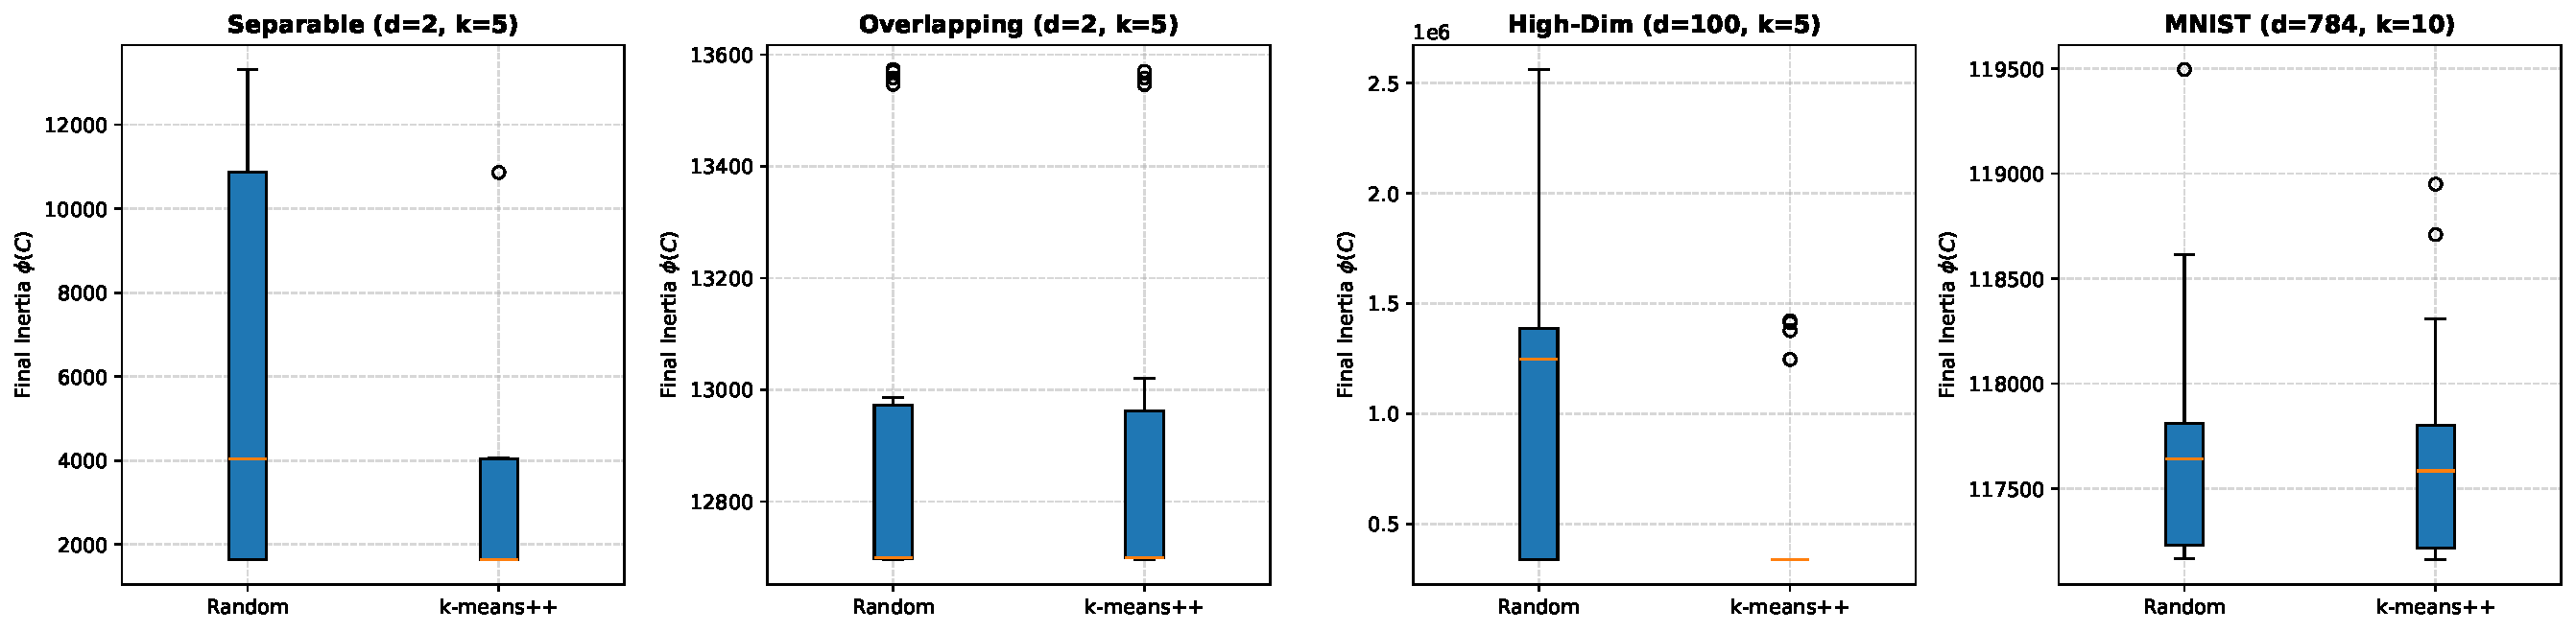
\includegraphics[width=\textwidth]{figures/inertia_distributions.pdf}
\caption{Final inertia distributions over 60 starts. Each panel compares the two initialisation choices on one dataset.}
\label{fig:inertia}
\end{figure}
\begin{figure}[H]
\centering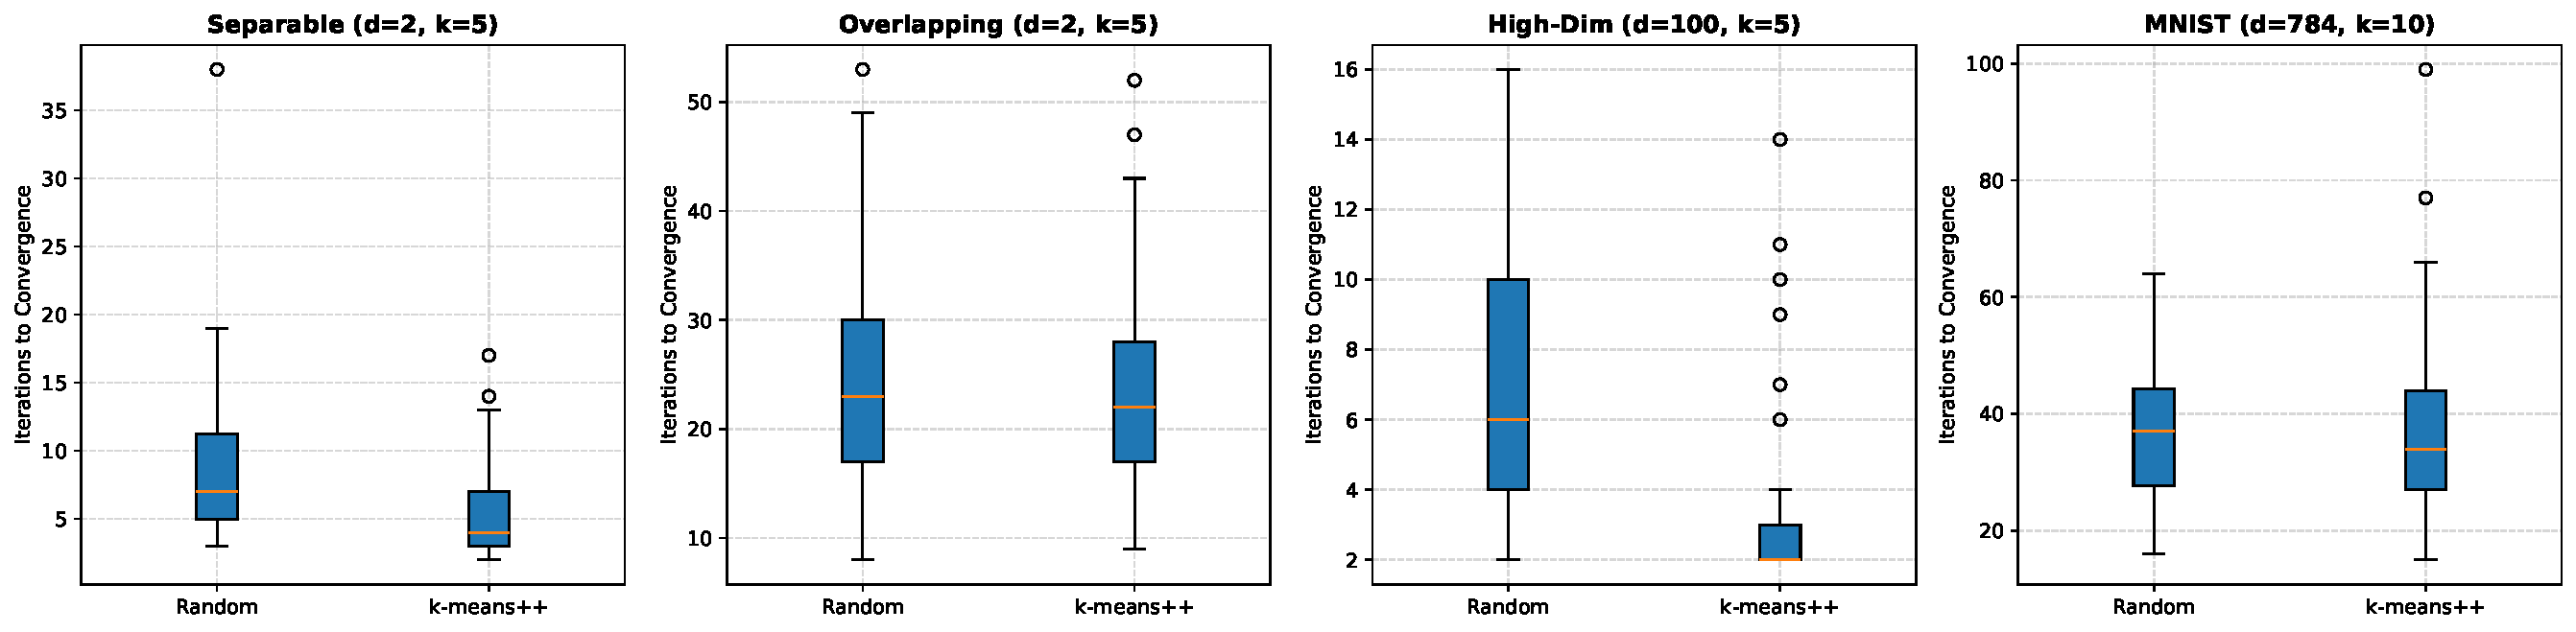
\includegraphics[width=\textwidth]{figures/convergence_iterations.pdf}
\caption{Number of Lloyd iterations to the centre-shift stopping criterion.}
\label{fig:iterations}
\end{figure}
\begin{figure}[H]
\centering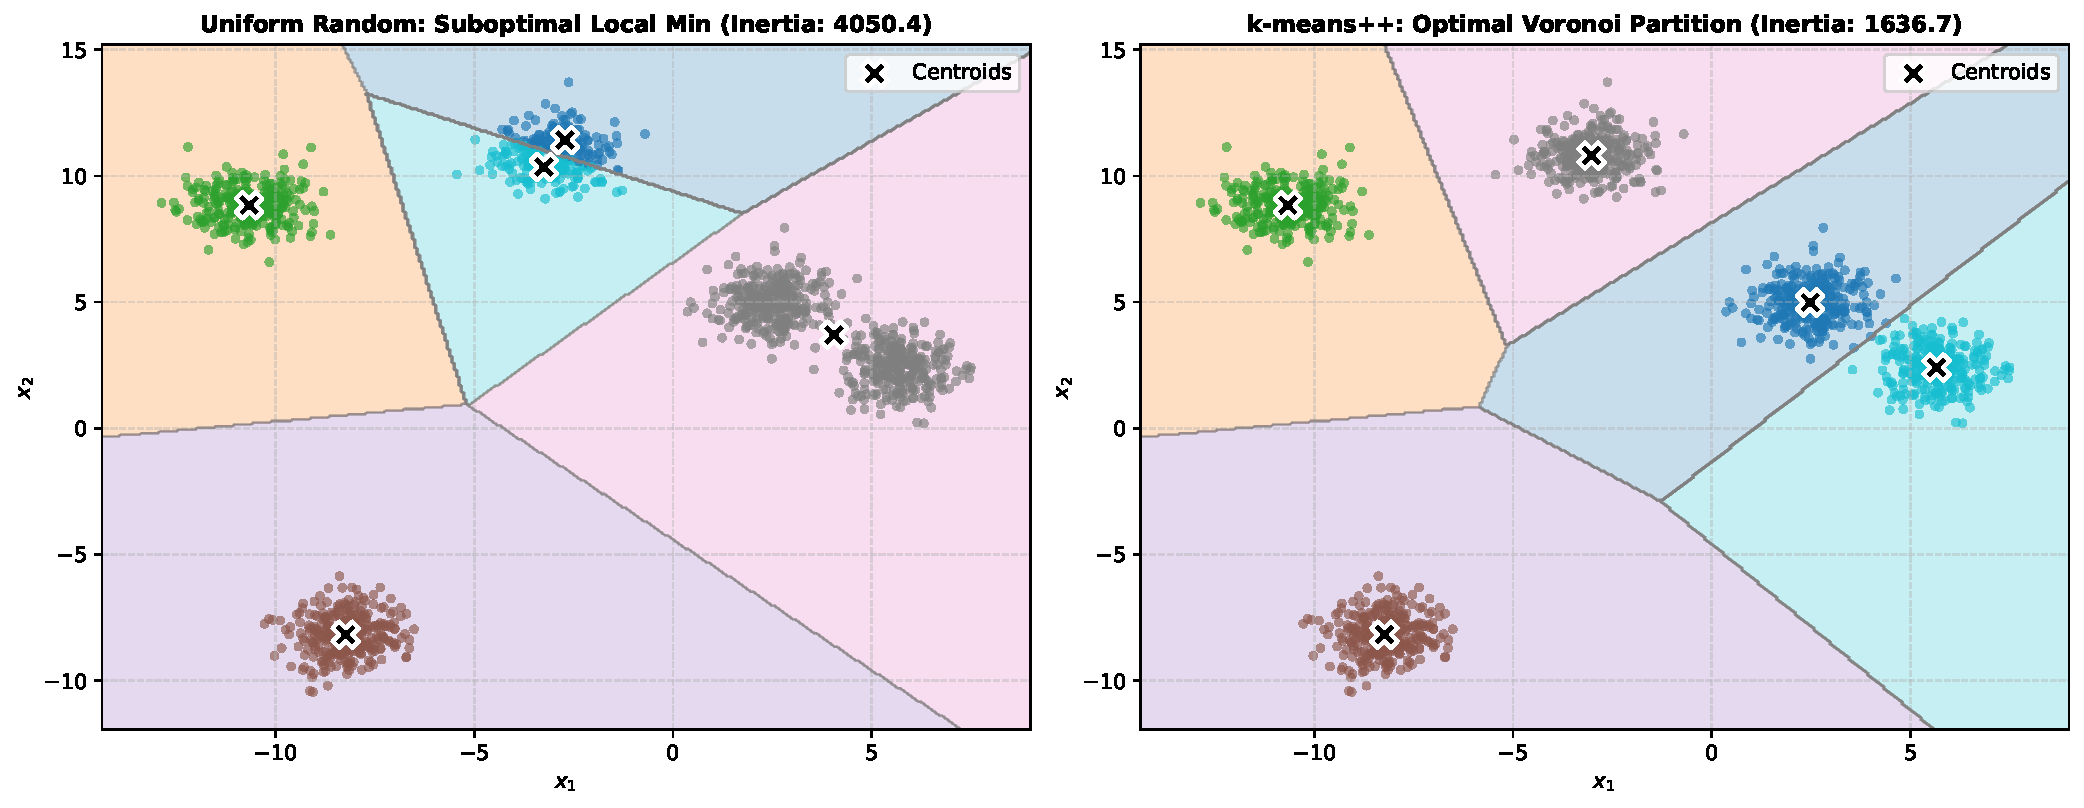
\includegraphics[width=0.9\textwidth]{figures/voronoi_comparison.pdf}
\caption{Separated two-dimensional example: a representative random-init local minimum (inertia about 4,050) and the lowest-inertia k-means++ outcome (inertia 1,636.7). The region colours are Voronoi assignments.}
\label{fig:voronoi}
\end{figure}

On separated blobs, mean inertia falls by about 48.8\% with k-means++, mean iterations fall by 38.3\%, and mean pairwise ARI rises from 0.753 to 0.857. External ARI and NMI also rise (0.822 to 0.903 and 0.910 to 0.950, respectively), indicating better correspondence to the known generated components in these runs. Random initialisation has a wide distribution, including runs above 13,000 inertia; k-means++ also has occasional poor outcomes, which is why its guarantee must not be interpreted deterministically. Figure~\ref{fig:voronoi} illustrates a split/merge local-minimum failure: an initialisation can use multiple centres for one true component and leave another component poorly represented. The best observed inertia, 1,636.7, is reached by both methods in some runs, consistent with a shared attainable solution.

On the overlapping data, mean inertia differs by only about 0.1\% (k-means++ lower), and iteration counts, stability, and external label scores are nearly identical. External ARI is about 0.55, lower than for the separated case, consistent with the designed overlap making component recovery harder. The broad overlap means the objective's best partition can be less aligned to the generating component labels; changing seeds alone does not remove this ambiguity. On the 100-dimensional data, mean inertia is about 50.3\% lower under k-means++, iterations are about half, stability rises from 0.687 to 0.904, and external ARI rises from 0.814 to 0.949. The k-means++ interquartile range is zero in this saved sample even though its full range is not: 49 of 60 runs reached the minimum observed inertia, while a minority reached worse minima. This concentration is consistent with, but does not prove, more reliable seeding in this generated geometry.

On MNIST, the mean inertia improvement is about 0.034\%, with a non-significant one-sided test and a bootstrap interval spanning zero. Mean iterations are slightly higher for k-means++, and the recorded mean wall times in this run are 501 ms for k-means++ and 468 ms for random initialisation. An earlier run had the reverse ordering, illustrating that runtime on this shared, parallel environment is noisy; it is not evidence for a reliable speed advantage. External ARI and NMI are modestly higher for k-means++ (0.381 vs 0.378 and 0.502 vs 0.497), but these are descriptive averages and no significance test was performed on them. Neither partition strongly recovers the digit labels. The modest inertia gap is plausible because the raw pixel Euclidean objective is not the same as digit recognition: within-digit handwriting variation and between-digit similarities can make class structure poorly represented by spherical clusters.

\subsection{Comparison with expected behaviour}
The experiments broadly match the expectation that k-means++ improves robustness on data where random seeding can create poor partitions. The strongest evidence is the substantial reduction in both average inertia and its dispersion on separated and high-dimensional blobs. The result is not universal: for overlapping blobs and MNIST, mean improvements are small and the rank-based test does not reject the no-directional-difference null at the chosen threshold. k-means++ is a probabilistic initialisation strategy, not a cure for model mismatch, overlapping distributions, or local optima. Consequently, the measured outcomes are consistent with the theory's expected initial-potential advantage while illustrating the gap between an expected seeding bound and finite-run final performance.

\section{Reproducibility, limitations, and conclusion}
The report's final tables were generated by the 60-trial runner, not by the notebook's earlier exploratory 30-trial runs on synthetic data. The runner records its local execution time, Python, NumPy, SciPy, scikit-learn, joblib, and Matplotlib versions, the MNIST cache timestamp, and bootstrap seed settings in the \texttt{\_metadata} entry of \texttt{experiments/results.json}. The results reported here were run on Python 3.12.4, NumPy 2.5.4, SciPy 1.18.1, scikit-learn 1.9.1, joblib 1.6.0, and Matplotlib 3.11.2.

From the project root, install the dependencies listed in \texttt{requirements.txt}. Then run:
\begin{lstlisting}
python experiments/run_experiments.py
python experiments/plot_results.py
\end{lstlisting}
The first command writes \texttt{experiments/results.json}; the second regenerates the report figures, including the notebook-matched PCA/t-SNE plot. OpenML access is needed on the first MNIST fetch unless its cache is already present. The random seeds, subset size, preprocessing, cluster counts, and trial counts are specified in the source files. Runtime values can vary by machine.

Limitations include the use of one generated sample per synthetic configuration, one fixed MNIST subset, and a fixed $k$ rather than a model-selection procedure. The external ARI/NMI scores give a label-based check but do not imply that digit categories are spherical or that this objective is ideal for image recognition. The tests and bootstrap intervals treat trial outcomes as uncertainty over initialisation on fixed data; they do not capture dataset-to-dataset uncertainty. The local cache timestamp records filesystem metadata, not the original publication or a verified download log for MNIST. No train/test split is used because the benchmark is clustering rather than prediction. A future extension could repeat data generation and subset selection with multiple seeds and compare additional scalings or dimensionality-reduction choices.

In conclusion, the from-scratch implementation exhibits Lloyd's expected monotone objective optimisation to a local solution, and the controlled repeated-start experiments show that k-means++ is notably advantageous on the two synthetic configurations with the largest observed local-minimum penalty. Its benefit is small and statistically inconclusive for overlapping blobs and this MNIST subset. The negative findings matter: initialisation cannot compensate for ambiguous geometry, and a visually or numerically stable partition does not by itself establish meaningful semantic clusters.

\section*{Declaration}
\addcontentsline{toc}{section}{Declaration}
\begin{quote}\small
I declare that this material, which I now submit for assessment, is entirely my own work and has not been taken from the work of others, save and to the extent that such work has been cited and acknowledged within the text of my work. I understand that plagiarism, collusion, and copying are grave and serious offences in the university and accept the penalties that would be imposed should I engage in plagiarism, collusion or copying. This assignment, or any part of it, has not been previously submitted by me or any other person for assessment on this or any other course of study.
\end{quote}

\bibliographystyle{plain}
\bibliography{references}
\end{document}